% Wie werden die Informationen die Benutzer gezeigt und wie können sie diese manipulieren
\subsection{Wahl der Frontendtechnologie}
Das Frontend ist für die Datenvisualisierung zuständig und erleichtert dem Endbenutzer die Datenmanipulation.\\
In diesem Kapitel werden Angular und React für die Entwicklung des Frontends bewertet. Beide Technologien haben unter anderem die Vorteile, gut dokumentiert zu sein und große Entwicklergemeinschaften zu haben. Dies begünstigt den Lernprozess und verschleunigt mögliche Problembehebungen. Große Entwicklergemeinschaften, bestehend aus Einzelpersonen und Unternehmen entwickeln die Frameworks weiter, wobei Angular von Google und React von Meta (ehemals Facebook) betreut wird. Die Technologien sind komponentenbasiert, was ihre Testbarkeit erleichtert. Maßgeblich an der Wahl der Technologien zum Vergleich verantwortlich war ihre Popularität - sie belegen in diversen Ranglisten die ersten Plätze.\cite{SO01}

Folgende Kriterien wurden berücksichtigt:
\begin{itemize}
  \item
        Der Schwierigkeitsgrad, um die Technologie zu lernen. Eine einfachere Technologie erlaubt es, früher mit der Durchführung des Projektes anzufangen und spart so Zeit und Kosten und damit wiederum das finanzielle Risiko.
  \item
        Die Akzeptanz bei den Entwicklern und die Anzahl von heruntergeladenen NPM-Paketen. Vermehrte Nutzung von Paketen erhöht die Wahrscheinlichkeit, dass Probleme in diesen schnell identifiziert und gelöst werden.\cite{LIN1}
  \item
        Vorkenntnisse des Entwicklungsteams.
        %\item
        % Die Flexibilität des Frameworks.
        % Der Zwang, Probleme auf eine bestimmte Weise zu lösen, oder die Alternative, eigene Lösungswege zu finden.

        %  \item
        %  Anzahl der ungelösten Probleme\footnote{Open issues}. 
\end{itemize}

\subsection{Angular}
\paragraph{}
Angular ist das Framework von Google für Mobil- und Webanwendungen.
\\
%STIMMT DAS? Angular lässt weniger Spielraum für eigene Entscheidungen darüber, wie der Code entwickelt wird. Deshalb eignet sich Angular besser für Projekte, wo mehrere Entwickler zusammenarbeiten. 

%Der Code wird mit Angular nach der Ri in einer vorgegebenen Art geschrieben werden sollte, um Einheitlichkeit zu schaffen.

Zu beachten ist, dass Angular nicht JavaScript als Hauptprogrammiersprache verwendet, sondern TypeScript.
TypeScript ist ein striktes Superset von ECMAScript 2015.
TypeScript muss erstmal kompiliert werden, um auf dem Browser laufen zu können{\cite{MS1}}. 

Dieses Framework ist besonders geeignet für fortgeschrittene, umfangreiche Projekte\footnote{{\cite{AN1}}, Seite 30}.
%CHECK THIS
%https://merehead.com/blog/angular-vs-react-vs-vue-best-choice-2022/

\subsection{React}
React ist eine Frontend-Technologie für die Entwicklung von Benutzeroberfläche für das Web und mobile Endgeräte\footnote{Mithilfe von React-Native} \cite{GH08}. 

React benutzt JSX, welche eine HTML-ähnliche Syntax hat.
Es wird empfohlen React-Komponenten mit JSX zu schreiben. 
Für die Verwendung von JSX ist ein Compiler erforderlich, der den JSX-Code in reines JavaScript umwandelt \footnote{{\cite{E01}, Seite 33}}.

Es besteht jedoch die Möglichkeit, diese in reinem JavaScript zu schreiben\cite{JSX1}.
\\
JSX ist eine JavaScript-Erweiterung.
Diese bietet die Möglichkeit Code zu schreiben, die einfach zu lesen und zu schreiben ist. 
Die Verwendung von JSX hat unter anderem den Vorteil, die Verhinderung von XSS-Angriffe\footnote{Cross Site Scripting{\cite{OWASP}}} \cite{JSX1}.
%\\\\
%Laut einer StackOverFlow Umfrage hat React.js im Jahr 2021 jQuery als das am häufigsten verwendete Web-Framework überholt. {\cite{SO01}}

%Die Entwicklung mit Angular hätte mehr Zeit und Lernaufwand gekostet. Außerdem ist das Projekt nicht komplex genug, um das Angular-Ökosystem zu benötigen.

\subsection{Lernkurve}
Im Vergleich zu React ist Angular komplex und hat eine steile Lernkurve {\cite{E01}}. 
\begin{quote}
  „Beispielsweise werden je nach Entwicklungsart bis zu fünf Dateien für eine einzelne Komponente benötigt, es müssen Abhängigkeiten eingefügt und die Komponenten in Modulen hinzugefügt werden. Infolgedessen wird ein Großteil der Entwicklungs-zeit in Angular für sich wiederholende Aufgaben aufgewendet.”
  \footnote{{\cite{AN1}, Seite 33}}
\end{quote}
Der Lernaufwand und die Entwicklung mit Angular beansprucht daher mehr Zeit, als die mit React.

\subsection{Popularität}
Folgende Indikatoren sind wichtig, denn je mehr Menschen an einem Open-Source-Projekt beteiligt sind, desto mehr Menschen tragen dazu bei, Fragen zu beantworten und Probleme beim Quellcode zu lösen {\cite{LIN1}}.
\\
Im folgenden wird die Beliebtheit und die Nutzung von React und Angular anhand von verschiedenen metriken betrachtet.

\begin{flushleft}
  \textbf{Developer Survey 2021 - StackOverFlow}\\
  StackOverFlow ist die größte Gemeinschaft von Softwareentwicklern, wo Wissen und Fragen zur Softwareentwicklung ausgetauscht wird.

  Seit 2011 führt StackOverFlow eine jährliche Umfrage zur Softwareentwicklung durch.

  \begin{figure}[h]
    \centering
    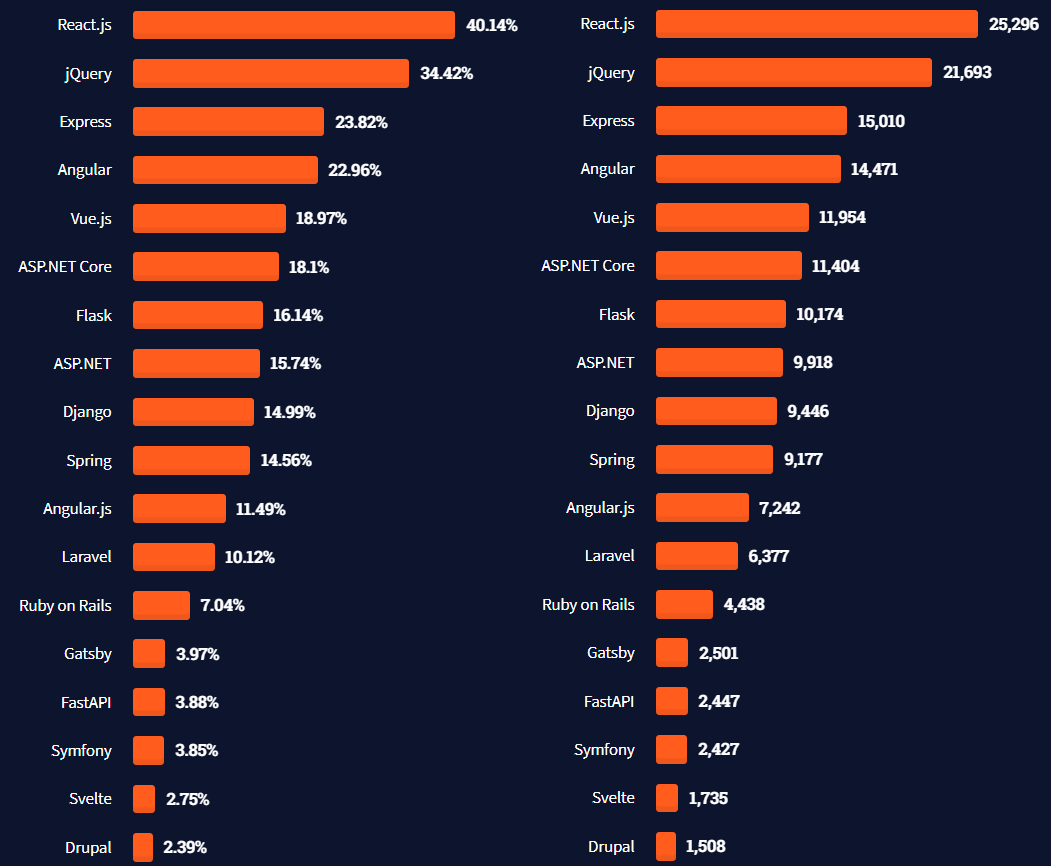
\includegraphics[scale=0.5]
    {Most popular Web Frameworks [Both] 2021.png}
    \caption{ Which web frameworks and libraries have you done extensive development work in over the past year, and which do you want to work in over the next year? (If you both worked with the framework and want to continue to do so, please check both boxes in that row.) {\cite{SO01}}}

  \end{figure}
\end{flushleft}

\newpage
\begin{flushleft}
  \textbf{Github}\\
  GitHub es ist eine Plattform für die Versionskontrolle von Source-Code, auf der mehr als 238 Millionen Repositories\footnote{Ablage für Quellcode gespeichert wird} verwaltet werden{\cite{GH07}}.
\end{flushleft}

Die Anzahl der Repositories, in denen Code für Angular und React gespeichert wird, gibt einen Hinweis auf die Beliebtheit dieses Frameworks.
\\
\begin{table}[b]
  \centering
  \begin{tabular}{ |p{5cm}||p{3.6cm}|p{3.6cm}|  }
    \hline
    \multicolumn{3}{|c|}{Github Statistiken}\\
    \hline 
    & Angular/core & React\\
    \hline
    Anzahl von Repositories & 2,011,663& 7,868,546
    \\
    \hline
    Sterne & 77.2k & 170k
    \\
    \hline
  \end{tabular}
\end{table}
{\cite{GH04, GH06}}
%https://risingstars.js.org/2020/es#section-statemanagement
%https://www.freecodecamp.org/news/angular-react-vue/
\begin{flushleft}
  Sterne werden auf Github verwendet, um die Beliebtheit eines Repositorys anzuzeigen.

  \newpage
  \textbf{NPM Paketen}\\
  Mithilfe von NPM werden die Abhängigkeiten eines Angular oder React Projekts verwaltet.

  Die Anzahl der heruntergeladenen NPM-Pakete gibt einen Hinweis auf die Nutzung der Technologie.
\end{flushleft}

\begin{center}
  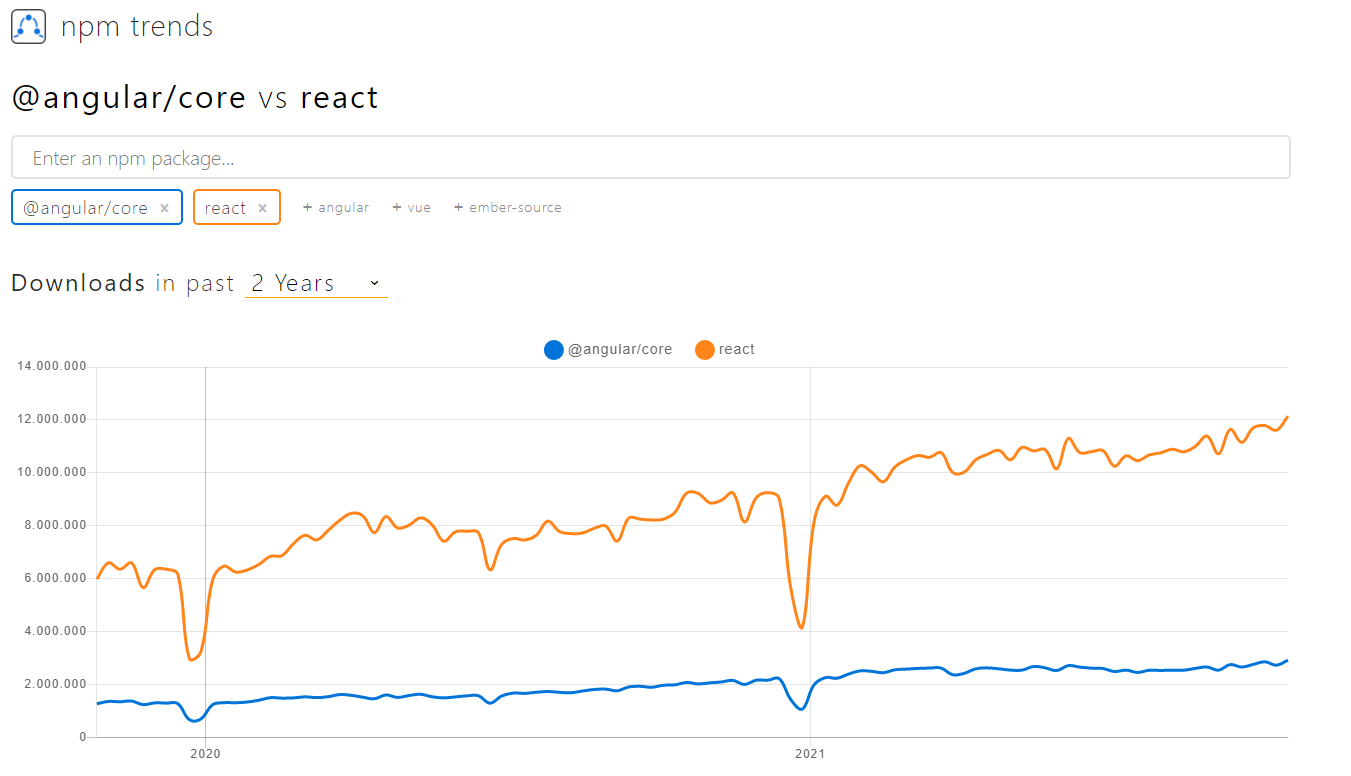
\includegraphics[scale=0.4]
  {sources/NPM-Trends React_Angular}\label{fig:NPM-Trends React_Angular}\\
  \textbf{Abbildung \autoref{fig:NPM-Trends React_Angular}:} heruntergeladenen NPM-Pakete \\@angular/core vs react
    {\cite{NPM01}}
\end{center}

%\newpage

\begin{flushleft}
  \textbf{Google Trends}\\
  In Zeitraum zwischen 01.11.2020 und 26.10.2021 wurde nach React häufiger als nach Angular gesucht. Dies belegen die Daten von GoogleTrends.
  %ein ganzes Jahr
  \\
  Diese Metrik ist ein weiterer Aspekt für die Beliebtheit des Frameworks.
\end{flushleft}

\begin{center}
  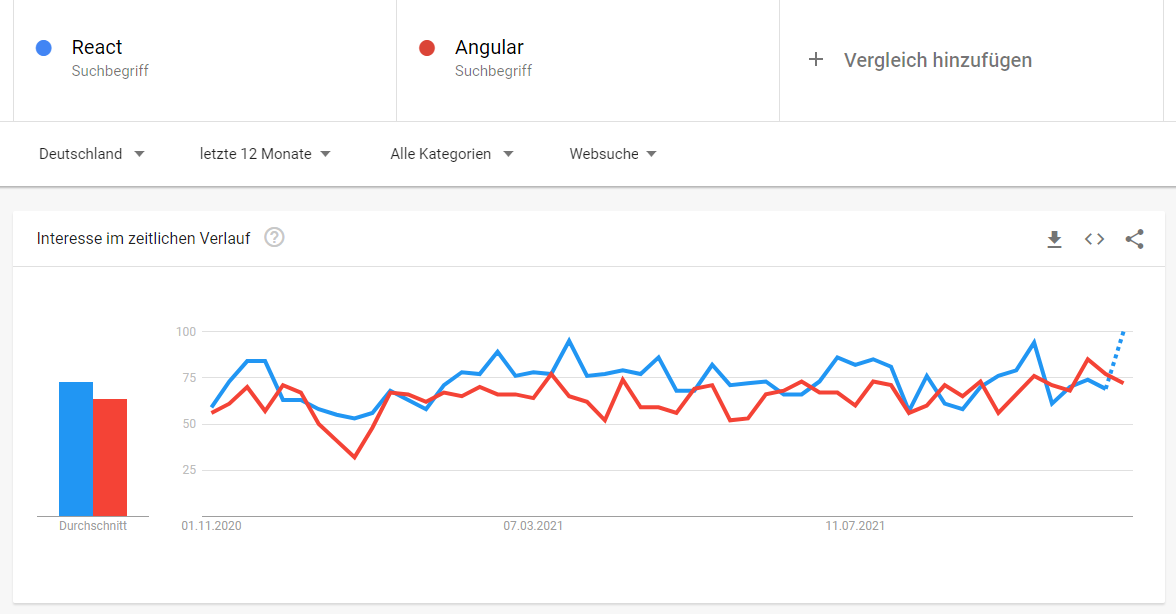
\includegraphics[scale=0.5]
  {sources/GoogleTrends React Angular 1.11.2020 29.10.2021}\label{fig:GoogleTrends React Angular 1.11.2020 29.10.2021}\\
  \textbf{Abbildung \autoref{fig:GoogleTrends React Angular 1.11.2020 29.10.2021}:} Google Trends Angular vs React
    {\cite{GO01}}
\end{center}


  \textbf{Jobangebote}\\
  \paragraph{}
  Als angehende Informatiker sind berufliche Perspektiven relevant, deswegen wurde den Arbeitsmarkt in der Entscheidungsfindung berücksichtigt.
  \\
  %In der Entscheidungsfindung sind ebenfalls künftige Perspektiven relevant.
  %Aus diesem Grund ist als angehende Informatiker den Arbeitsmarkt berücksichtigt.   
  Anzahl der Jobangebote bei LinkedIn in Deutschland:
  \\
  Angular: 7.657 Ergebnisse{\cite{LI1}}
  \\
  React: 11.523 Ergebnisse{\cite{LI2}}

\subsection{Vorkenntnisse}
Das Entwicklungsteam verfügt über Javascript-Kenntnisse, was für die Wahl einer Technologie wie React spricht, die keine neuen Kenntnisse erfordert. Das vorhandene Wissen wird die Entwicklungszeit beschleunigen und Weiterbildungskosten vermeiden.

\subsection{Fazit}
Es ist anzumerken, dass die Entwicklung des Projekts mit jedem der beiden Frameworks möglich ist.
\\
%Die Vorkenntnisse des Entwicklerteams und der Anzahl an Jobangeboten haben in diesem Projekt für React eine bedeutende Rolle gespielt. FERTIG?
Bei der endgültigen Entscheidung wurde React aufgrund ihrer geringen Lernkurve, ihrer guten Zustandsverwaltung\footnote{State Management}, ihre große Popularität und ihrer Einfachheit berücksichtigt.
Die folgende Abbildung fasst die wichtigsten Unterschiede und Gemeinsamkeiten zwischen React und Angular zusammen.
  \begin{center}
    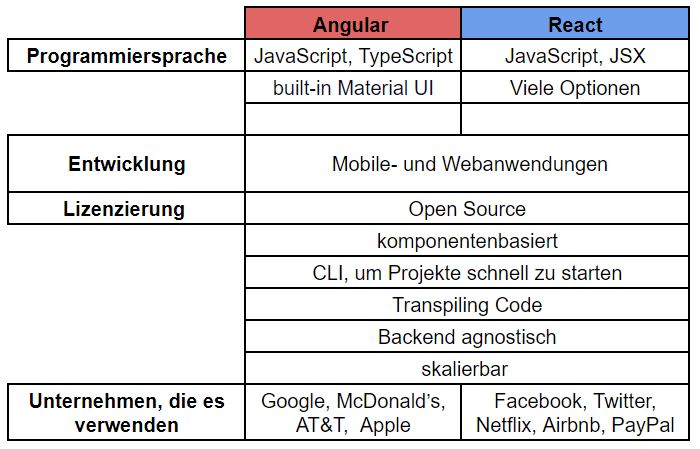
\includegraphics[scale=0.7]
    {sources/Angular_vs_React}\label{fig:Angular_vs_React}\\
    \textbf{Abbildung \autoref{fig:Angular_vs_React}:} 
    Vergleich Angular vs React
     % {\cite{GO01}}
  \end{center}


\subsection{React Hooks}
%https://www.javatpoint.com/react-hooks
Beginnend mit 16.8.0, enthält React eine stabile Implementierung von React Hooks.

Ab dieser Version wird React empfohlen, keine Klassen mehr für die Erstellung von Komponenten zu verwenden.
Mit Klassen geschriebene Komponenten werden weiterhin unterstützt und müssen nicht neu geschrieben werden.
  {\cite{R05}}
\\

\textbf{useState}
\\
Der Hook useState bietet die Möglichkeit an, den Zustand einer Anwendung zu verwalten.

In diesem Projekt wurde useState verwendet, um alle Benutzerdaten zu manipulieren und lokal zwischen zu speichern.

Nachdem der Klient eine gültige Abfrage an den Server gesendet hat, werden die Daten in den durch useState definierten Variablen gespeichert.
\begin{center}
  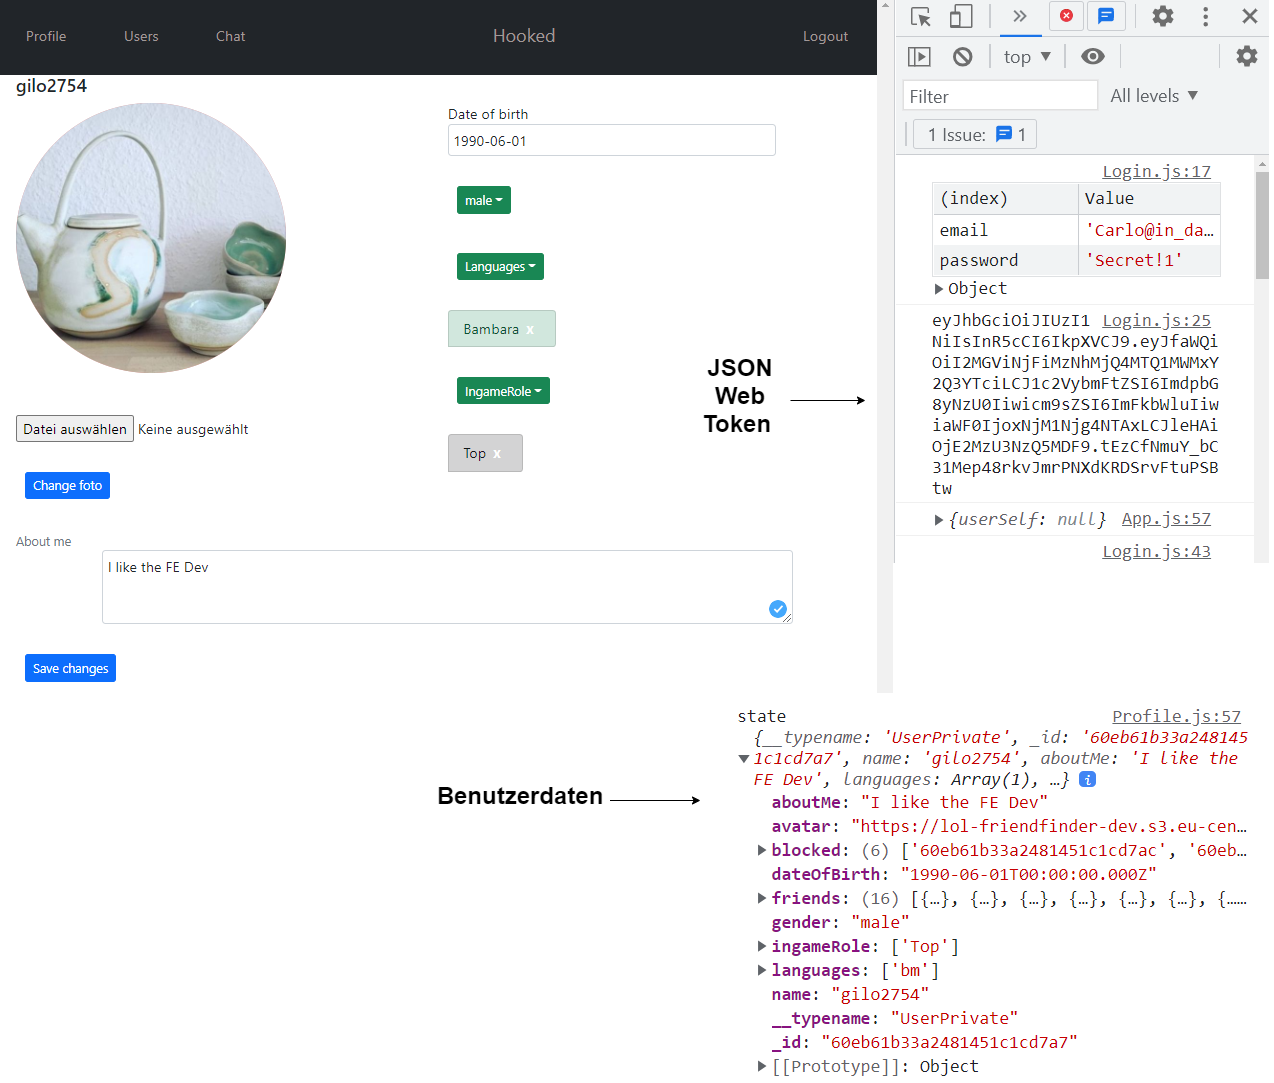
\includegraphics[scale=0.35]
  {sources/Server-Abfrage-Antwort}\label{fig:Server-Abfrage-Antwort}\\
  \textbf{Abbildung \autoref{fig:Server-Abfrage-Antwort}:} Server-Abfrage-Antwort
\end{center}

Die Abfrage an den Server für die Anmeldung gibt das JSON Web Token\\(Authentifizierungstoken){\cite{RFC7519}} zurück, das es dem Benutzer ermöglicht, eine aktive Sitzung aufrechtzuerhalten. Dieses Token wird für künftige Abfragen benötigt, um den Zugriff auf die Informationen des Nutzers zu ermöglichen.
\\
Eine genauere Funktionsweise der Serverabfragen folgt in Kapitel Serverabfragen.
\\
%In späteren Kapiteln wird näher erläutert, wie diese Informationen, die durch einen einzigen Abfrage an den Server erhalten werden, in den Chat- und Benutzerkomponenten genutzt werden.

%Wie man sieht, gibt es innerhalb des states nicht nur einen Wert, sondern mehrere.
%Es handelt sich eigentlich um ein Objekt. Objekte sind dasselbe wie Variablen in JavaScript, der einzige Unterschied ist, dass ein Objekt mehrere Werte in Form von Eigenschaften und Methoden enthält.
%Objekte können andere Objekte, Strings, Arrays, Zahlen und so weiter enthalten.
%\newpage

\textbf{useEffect}
\\
useEffect ermöglicht es, verschiedene Arten von Effekten zu erzeugen, nachdem eine Komponente gerendert wurde.

Unter Effekte sind zu verstehen, die Art und Weise, in der die Daten angezeigt werden. useEffect kümmert sich um die Aktualisierung des HTML-DOM\footnote{Document Object Model {\cite{MO2}}}, wenn dies erforderlich ist. Die Aktualisierung des HTML-DOM erfolgt auf Komponentenebene. Nur die Komponenten, die aktualisiert werden müssen, werden neu geladen.
\\
Dies ist möglich, indem  das virtuelle React-DOM{\cite{R06}} und das HTML-DOM im Browser vergliechen werden\footnote{{\cite{AN1}, Seite 22}}.
\\\\
Wenn der Benutzer Änderungen im Bereich Benutzerprofil vornimmt, werden diese erstmal in der Variable „state” zwischengespeichert, bevor sie in der Datenbank gespeichert werden.
\\
Die Abfrage zur Aktualisierung der Daten wird in dem Moment an den Server gesendet, in dem der Benutzer auf die Taste „Save/Speichern“ drückt.
\\
Zu diesem Zeitpunkt wird die Benutzeroberfläche durch useEffect aktualisiert, da sich die Variable „state” als Abhängigkeit von useEffect festgelegt ist und diese neue Informationen enthalten.
\\\\
Ein Beispiel dafür ist, wenn der Benutzer das Feld Sprachen aktualisiert. Beim Speichern der Änderungen werden nur die Komponente, die mit der vorgenommenen Änderung zusammenhängt, wieder in das HTML-DOM geladen.
\\\\

\textbf{useContext}
\\
useContext ermöglicht Daten innerhalb bestimmte Komponenten zu teilen.
In diesem Projekt war useContext eingesetzt, um die Benutzerdaten und den Authentifizierungstoken über die Komponenten  „Profile“, „Chat“, „Users“ zu teilen.
\\\\
UseContext bietet eine Lösung, um Daten zwischen Komponenten auszutauschen.{\cite{R04}}
\\
In diesem Projekt war es nötig, Daten über mehrere Komponenten zu teilen, weil die Benutzerdaten in mehrere Komponenten konsumiert wurden.

%\newpage
Zum Beispiel, die Kennung\footnote{User id} der Freunde eines Benutzers, sind in der Variable „state” enthalten. Diese Informationen werden in der Komponente „Chat” verwendet, um Einzelheiten über die Freunde des angemeldeten Benutzers bereitzustellen.

Zusätzlich befindet sich auch die Kennung der Nachrichten\footnote{Chat id} pro Benutzer. Diese wurde verwendet, um die Nachrichten abzufragen, die die Benutzer untereinander ausgetausch haben.
\begin{center}
  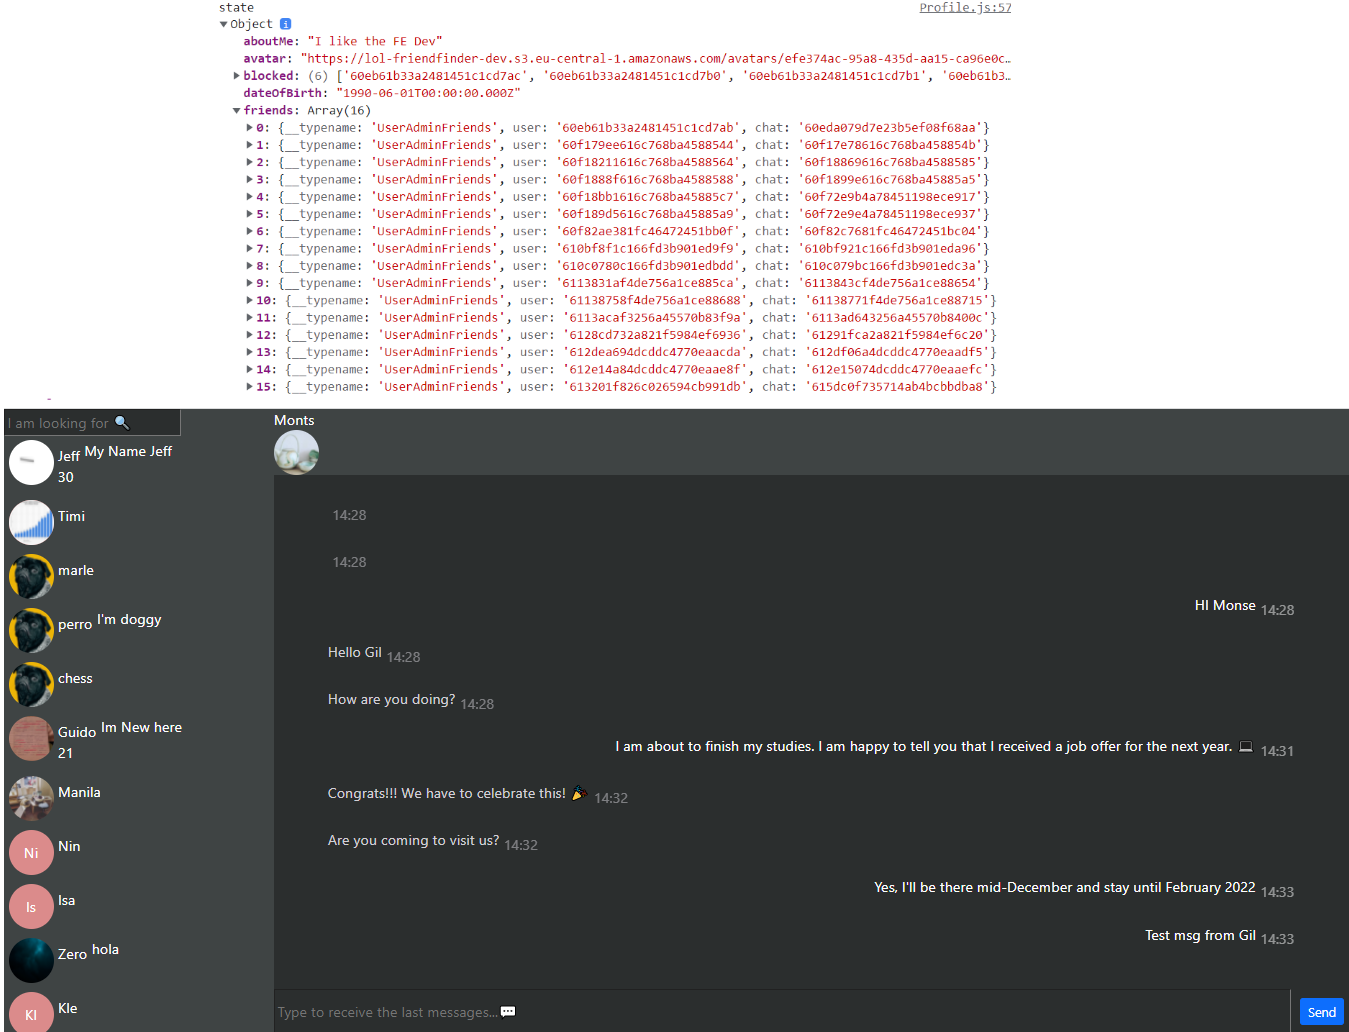
\includegraphics[scale=0.45]
  {sources/Friends_in_Chat}\label{fig:Friends_in_Chat}\\
  \textbf{Abbildung \autoref{fig:Friends_in_Chat}
    Einzelheiten der Freunden}
\end{center}


Im Anhang 5 und 6 befidet sich der Code mit dem den Authentifizierungstoken und die Benutzerdaten global  mithilfe von useContext verwaltet wird.

